\documentclass[12pt, a4paper]{article}

\usepackage{graphicx}
\usepackage{float}
\usepackage{tabularx}
\usepackage{booktabs}
\usepackage{hyperref}
\usepackage{amsmath}

\begin{document}
	\pagenumbering{gobble}
		\begin{titlepage}
			\centering
			{\LARGE Controls Systems Practical 7\par}
			\vspace*{1.5cm}
			{\large Q. Kruger, 216008466 \par}
			{\large R. de Bruyn, 216054484 \par}
			\vspace*{1.2cm}
			{\large \today}
			\vspace*{\fill}
			% 
\includegraphics[width=\textwidth]{img/UJ.jpg}
			\vspace*{\fill}
		\end{titlepage}

	\pagenumbering{roman}
	\tableofcontents
	\listoffigures
	\newpage
	\pagenumbering{arabic}

	\section{Prelab} % (fold)
	\label{sec:prelab}
		Possible sketches for the configuration in the practical guide are given below for different positions of the zeros relative to the poles

		\begin{figure}[H]
			\centering
			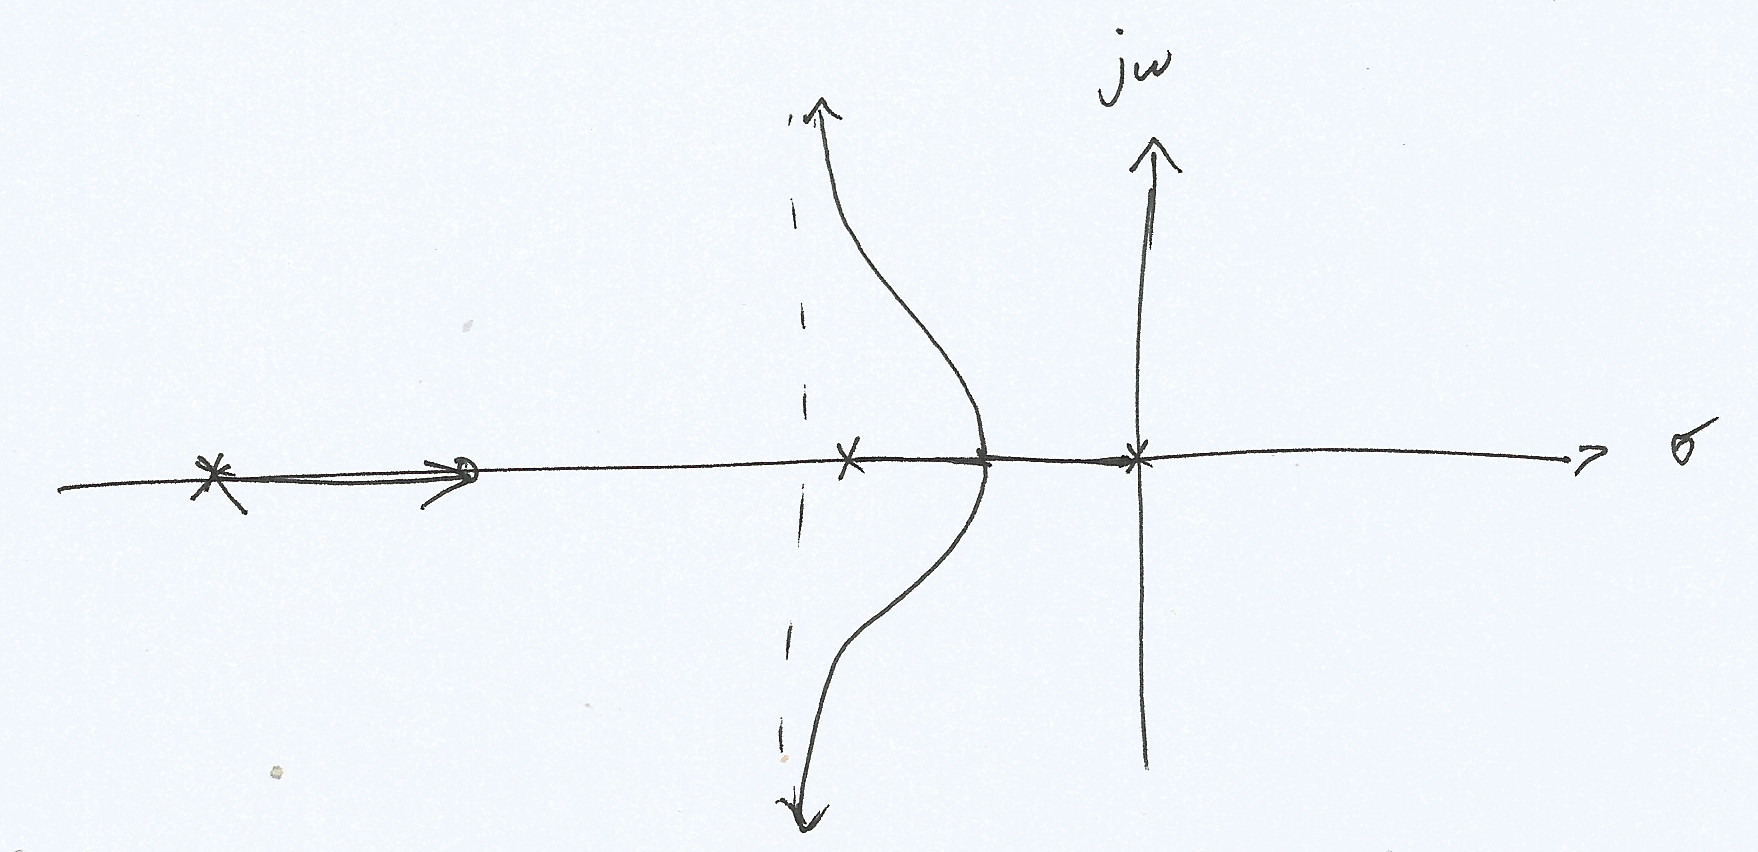
\includegraphics[width=\textwidth]{img/rlocus1.jpg}
			\caption{First configuration}
		\end{figure}
		
		\begin{figure}[H]
			\centering
			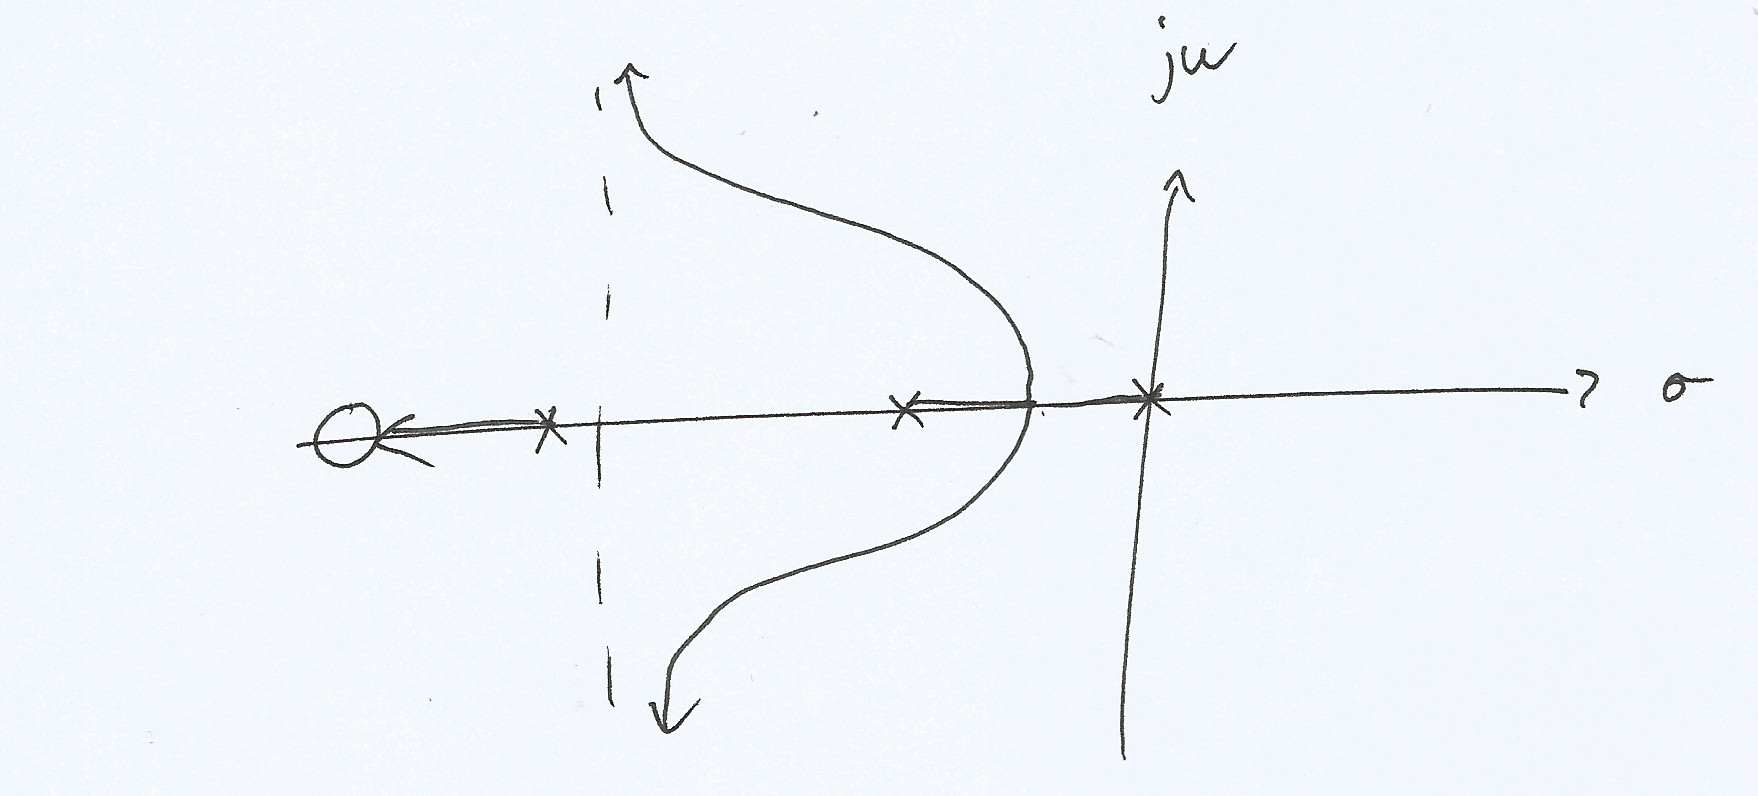
\includegraphics[width=\textwidth]{img/rlocus2.jpg}
			\caption{Second configuration}
		\end{figure}
	% section prelab (end)

	\section{Lab} % (fold)
	\label{sec:lab}
		For the first part of the lab, we have the a negative unity feedback loop system with function
		\begin{equation}
			G(s) = \frac{K(s+z)}{s(s+0.5)(s+10)}
			\label{eq:lab_1}
		\end{equation}

		\noindent with has a transfer of
		\begin{equation}
			T(s) = \frac{G(s)}{1 + G(s)}
			\label{eq:ts}
		\end{equation}

		Below we plot the root locus of the system given in \eqref{eq:lab_1} for $z=6,2,1.2$, and with $K=1$:

		\begin{figure}[H]
			\centering
			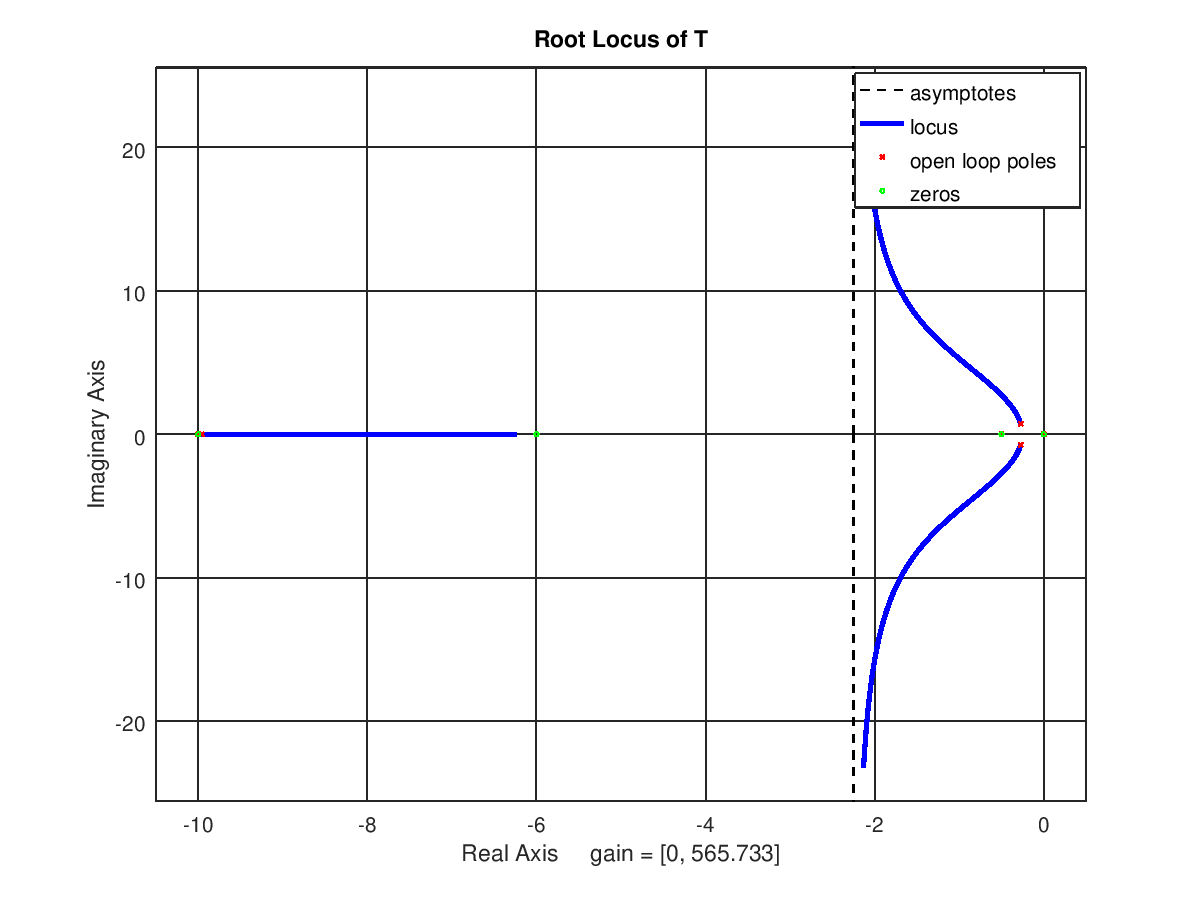
\includegraphics[width=.8\textwidth]{img/rlocus_1.png}
			\caption{Root locus of $G(s),\,z=6$}
			\label{fig:fig_1}
		\end{figure}

		\begin{figure}[H]
			\centering
			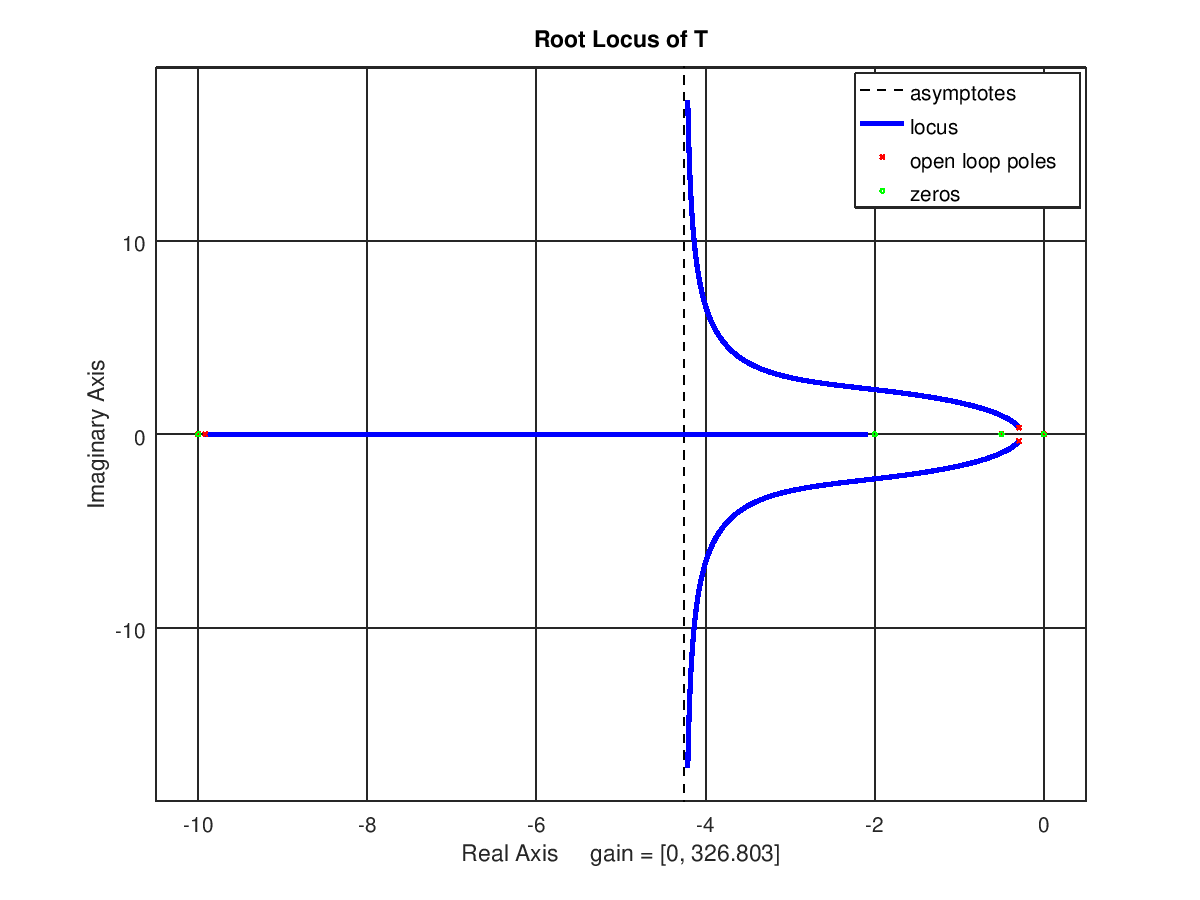
\includegraphics[width=.8\textwidth]{img/rlocus_2.png}
			\caption{Root locus of $G(s),\,z=2$}
			\label{fig:fig_2}
		\end{figure}

		\begin{figure}[H]
			\centering
			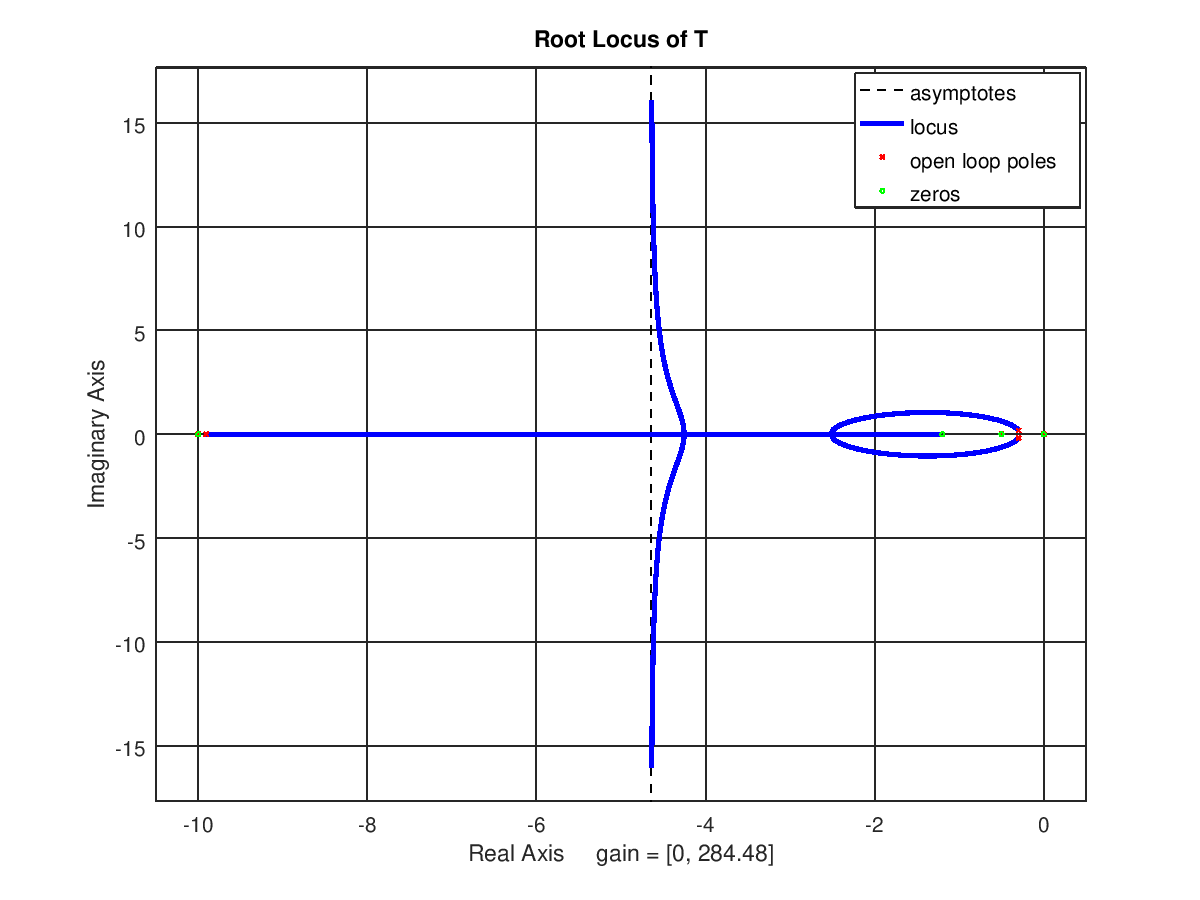
\includegraphics[width=.8\textwidth]{img/rlocus_3.png}
			\caption{Root locus of $G(s),\,z=1.2$}
			\label{fig:fig_3}
		\end{figure}

		For the second part of this practical, we consider the same system as in prelab 2, a negative unity feedback system with
		\begin{equation}
			G(s) = \frac{K(s+1.5)}{s(s+0.5)(s+10)}
			\label{eq:lab_2}
		\end{equation}

		Plotting the transfer function with the same expression as given in equation \eqref{eq:ts}, we have the following plots for $K=20, 200, 700$:
		\begin{figure}[H]
			\centering
			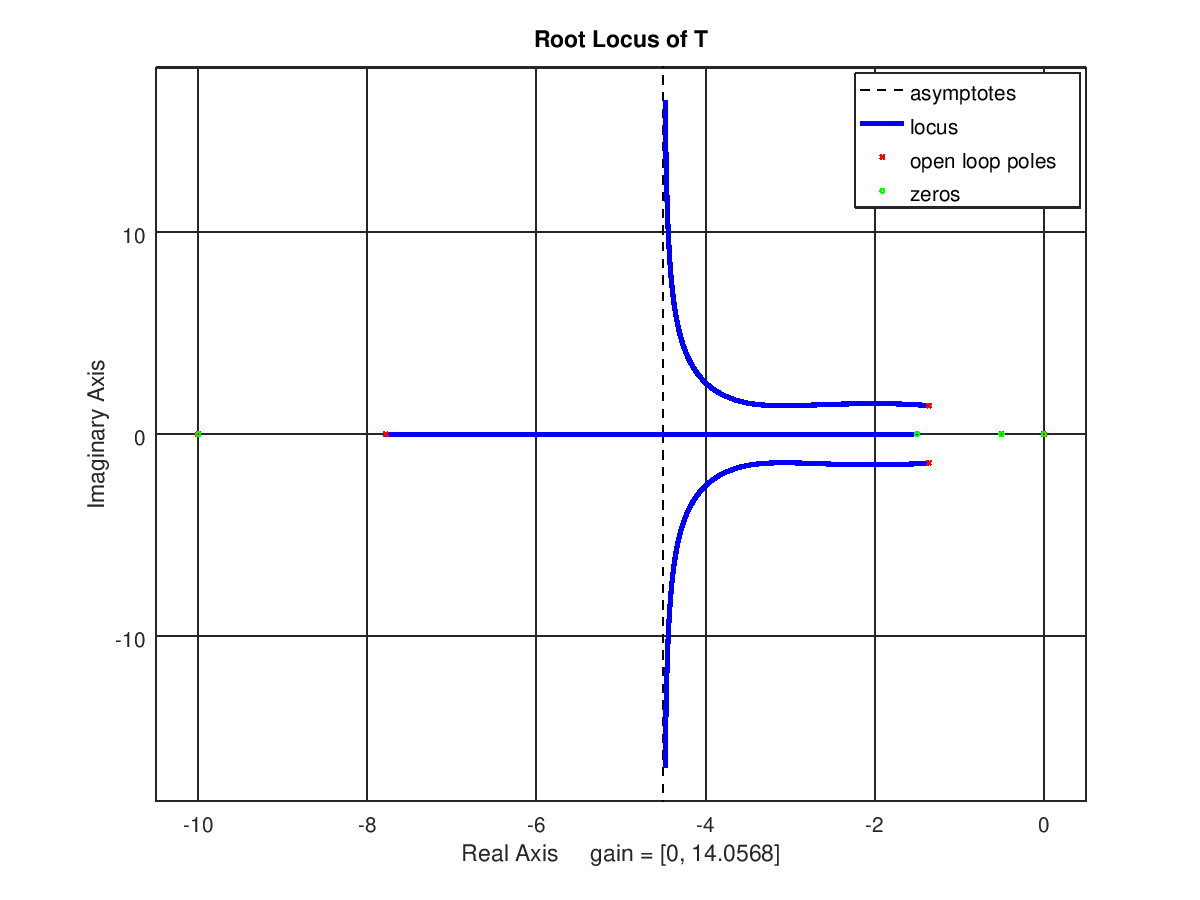
\includegraphics[width=.8\textwidth]{img/rlocus_20.png}
			\caption{Root locus for $K = 20$}
			\label{fig:rlocus_20}
		\end{figure}

		\begin{figure}[H]
			\centering
			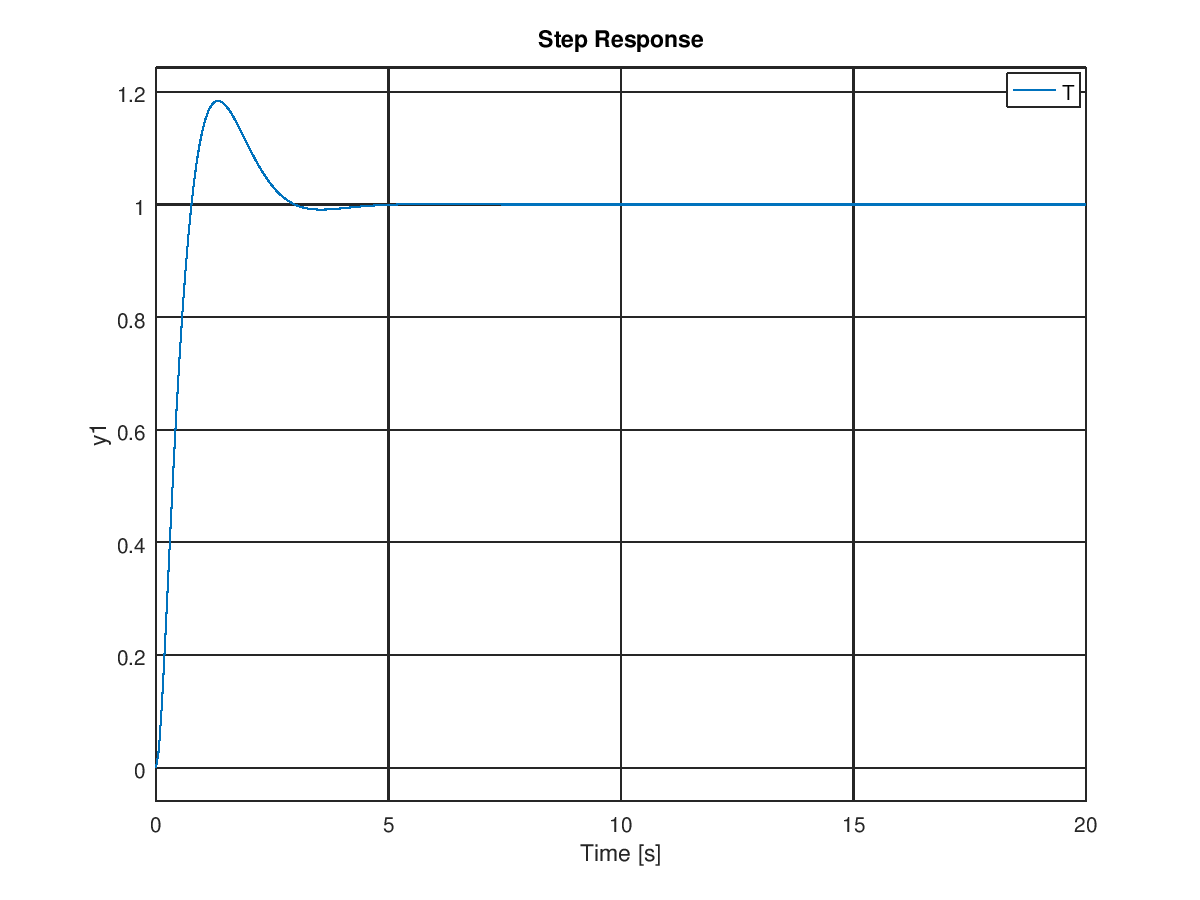
\includegraphics[width=.8\textwidth]{img/step_20.png}
			\caption{Step response for $K = 20$}
			\label{fig:step_20}
		\end{figure}

		\begin{figure}[H]
			\centering
			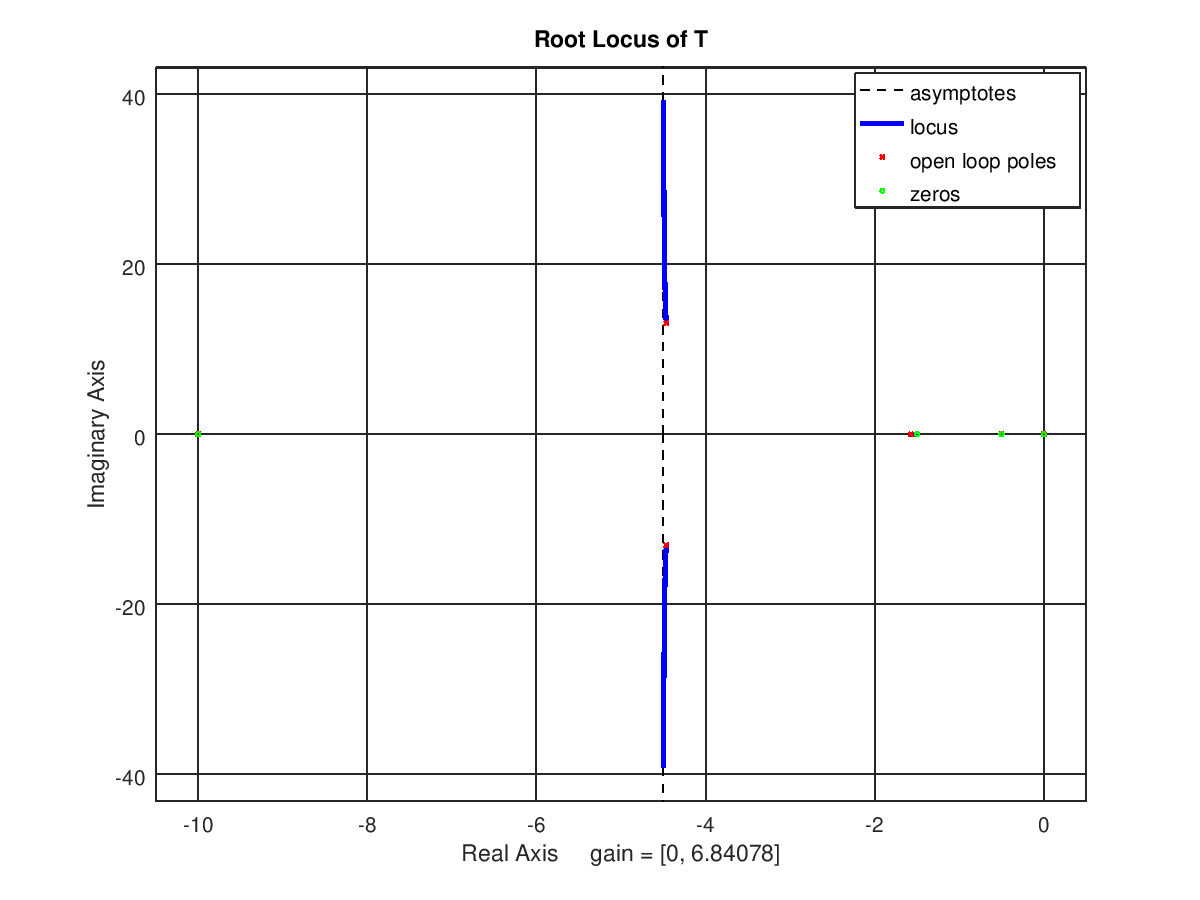
\includegraphics[width=.8\textwidth]{img/rlocus_200.png}
			\caption{Root locus for $K = 200$}
			\label{fig:rlocus_200}
		\end{figure}

		\begin{figure}[H]
			\centering
			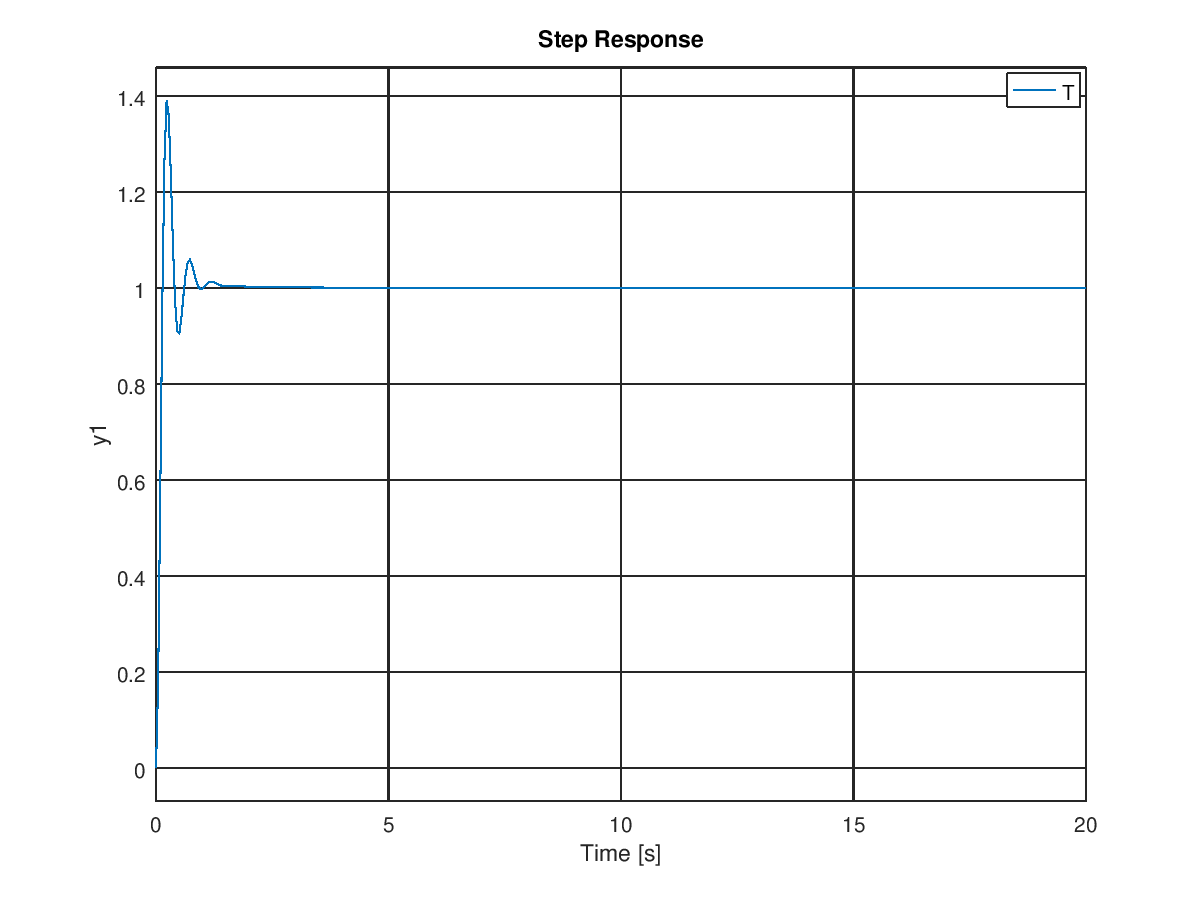
\includegraphics[width=.8\textwidth]{img/step_200.png}
			\caption{Step response for $K = 200$}
			\label{fig:step_200}
		\end{figure}

		\begin{figure}[H]
			\centering
			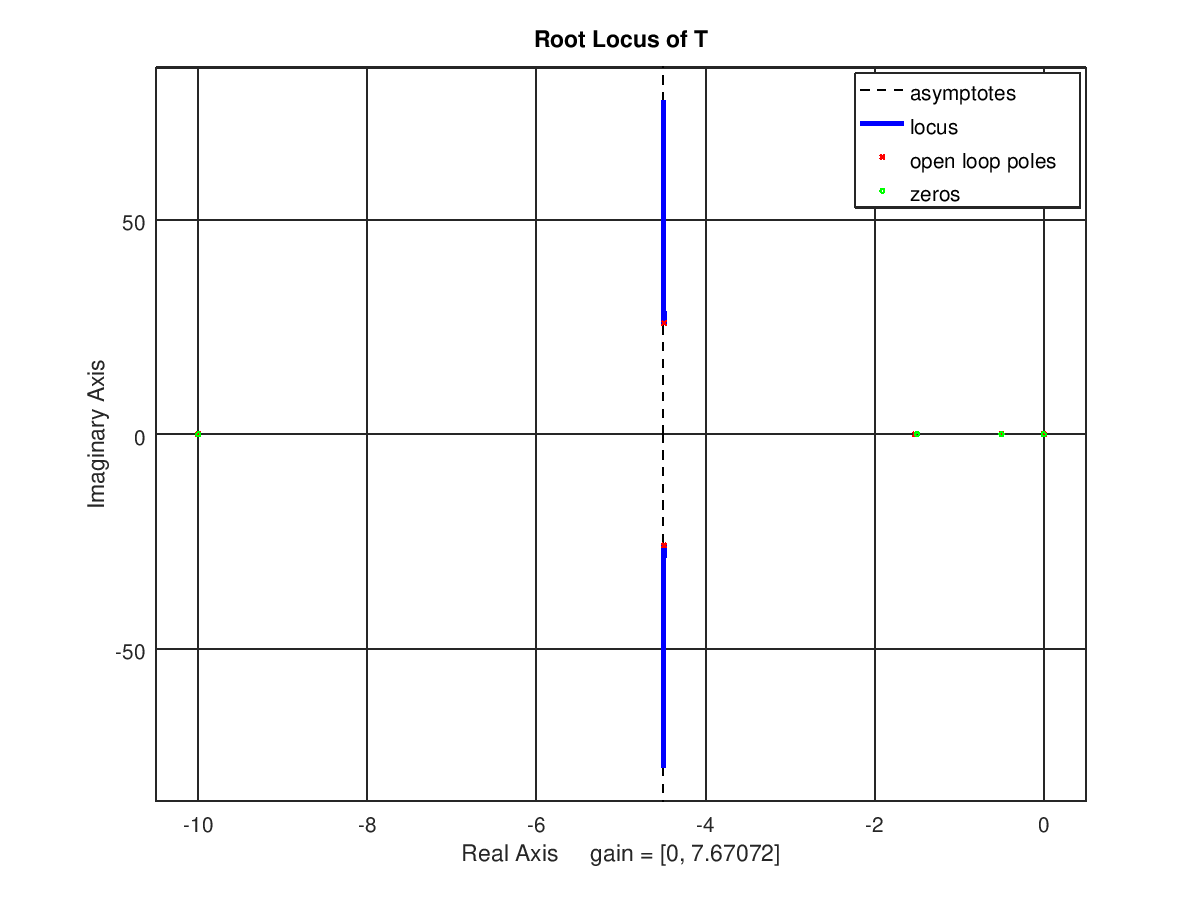
\includegraphics[width=.8\textwidth]{img/rlocus_700.png}
			\caption{Root locus for $K = 700$}
			\label{fig:rlocus_700}
		\end{figure}

		\begin{figure}[H]
			\centering
			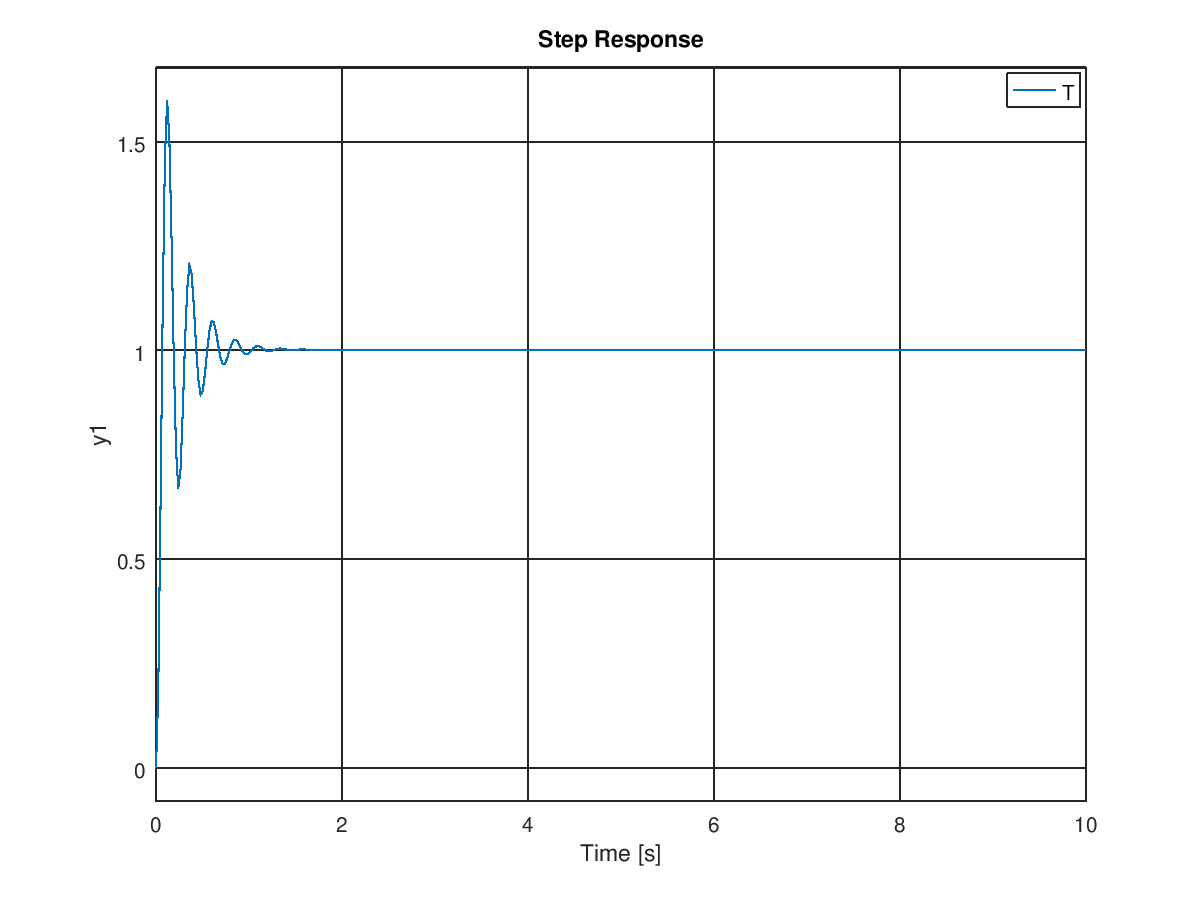
\includegraphics[width=.8\textwidth]{img/step_700.png}
			\caption{Step response for $K = 700$}
			\label{fig:step_700}
		\end{figure}
	% section lab (end)

	\section{Postlab} % (fold)
	\label{sec:postlab}
		From the results in the prelab and especially in the lab, we can see that the zeros have a very profound effect on the root locus and step response of the system. As from theory, changing the coordinates of a pole directly shifts the asymptotes of the system as well.

		The table below tabulates the results that we have obtained from the second part of the lab. Curiously, the settling time for $K = 700$ was slower than that for $K = 200$, even though we would expect that it would have a faster settling time.
		\begin{table}[H]
			\begin{tabularx}{\textwidth}{X X X}
				\toprule
				Gain & \%OS & $T_s$ \\
				\midrule
				20 & 18.4 & 2.64 \\
				200 & 38.9 & 0.84 \\
				700 & 59.7 & 0.87 \\
				\bottomrule
			\end{tabularx}
		\end{table}
	% section postlab (end)
\end{document}